

\subsection{Objetivos:}
    \begin{itemize}
        \item Diseño de la lógica de control de un ascensor.
        \item Implementación y validación de dicho diseño en lenguaje VHDL.
        \item Simulación de cada entidad implementada para verificar su funcionamiento mediante un testbench en código VHDL.
        \item Sintetizado sobre la tarjeta SPARTAN-3 Starter Kit del laboratorio
    \end{itemize}
    
\subsection{Funcionamiento general del Ascensor y requisitos:}

\subsection{Placa Spartan-3 Starter Kit Board} \label{subsection:Spartan-3}
    
    Para la implementación de este proyecto y si realización sobre un soporte físico real se utilizará la placa Spartan-3 Starter Kit Board de Xilinx, que incluye la FPGA así como otros componentes que nos vendrán bien a la hora de simular el comportamiento del ascensor.

    En las figuras que se muestran a continuación se pueden ver la distribución de los componentes del Kit:

    \begin{figure}[H]
            \centering
            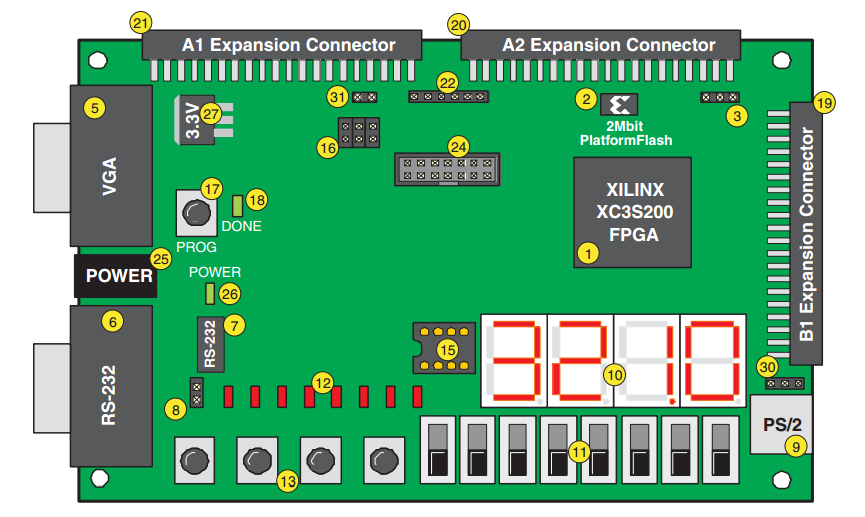
\includegraphics[width = 0.8\textwidth ]{Spartan3TopSide}
            \caption{Placa Spartan-3 (parte superior)}
            \label{fig:Spartan3TopSide}
    \end{figure}

    \begin{figure}[H]
            \centering
            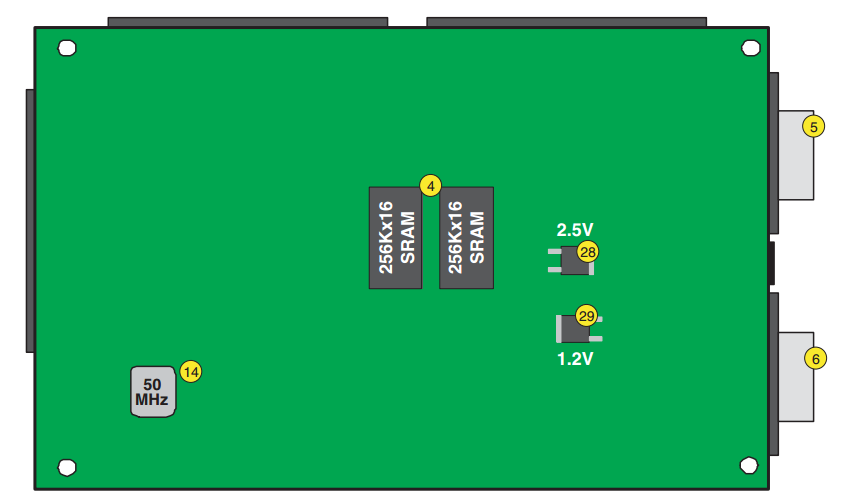
\includegraphics[width = 0.8\textwidth ]{Spartan3BottomSide}
            \caption{Placa Spartan-3 (parte inferior)}
            \label{fig:Spartan3BottomSide}
    \end{figure}

    Nos centraremos en los componentes más importantes que utilizaresmos para la realización de este proyecto:

    \begin{itemize}
        \item [1.] Xilinx Spartan-3 XC3S200 FPGA  (encapsulado XC3S200FT256). Compuesta por 200000 puertas.
        \item [2.] 2Mbit Xilinx XCF02S Platform Flash.
        \item [4.] 1M-byte of Fast Asynchronous SRAM.
        \item [10.] Cuatro displays LED de 7 segmentos.
        \item [11.] Ocho interruptores.
        %\item [12.] Ocho salidas LED independientes.
        \item [13.] Cuatro pulsadores.
        \item [14.] Cristal osculador (CLK) de 50MHz.
        \item [18.] LED indicador de que la FPGA ha sido configurada correctamente

    \end{itemize}

    Las salidas físicas para los \textbf{displays de 7 segmentos} se encuentran en los pines que se pueden ver en la siguiente tabla. Los displays se encuentran representados con el número 10 en la figura (\ref{fig:Spartan3TopSide}) del apartado (\ref{subsection:Spartan-3}). \\ 

    Como se puede ver en la figura los 4 displays comparten 8 pines de control, para elegir un display u otro están los Ánodos de control, en la tabla (\ref{tab:anodoControl}). \\ 

    Es importante tener en cuenta que los cuatro display de 7 segmentos comparten la entrada de 7 bits que codifica el caracter; se elige por que display se muestra dicha información sacando un valor de alto nivel por el ánodo de control correspondiente. \\ 

    \begin{table}[H]
            \centering
            \begin{tabular}{|c|c|c|c|c|c|c|c|c|}
                \hline
                \rowcolor[rgb]{0.21,0.69,0.87}\multicolumn{9}{|c|}{  \textbf{ {Salidas físicas Display 7 segmentos}}} \\
                \hline \hline
                \textbf{  Segmento  } & A & B & C & D & E & F & G & DP \\ 
                \hline
                \textbf{  FPGA Pin  }  & E14 & G13 & N15 & P15 & R16 & F13 & N16 & P16 \\ 
                \hline
                \multicolumn{9}{|c|}{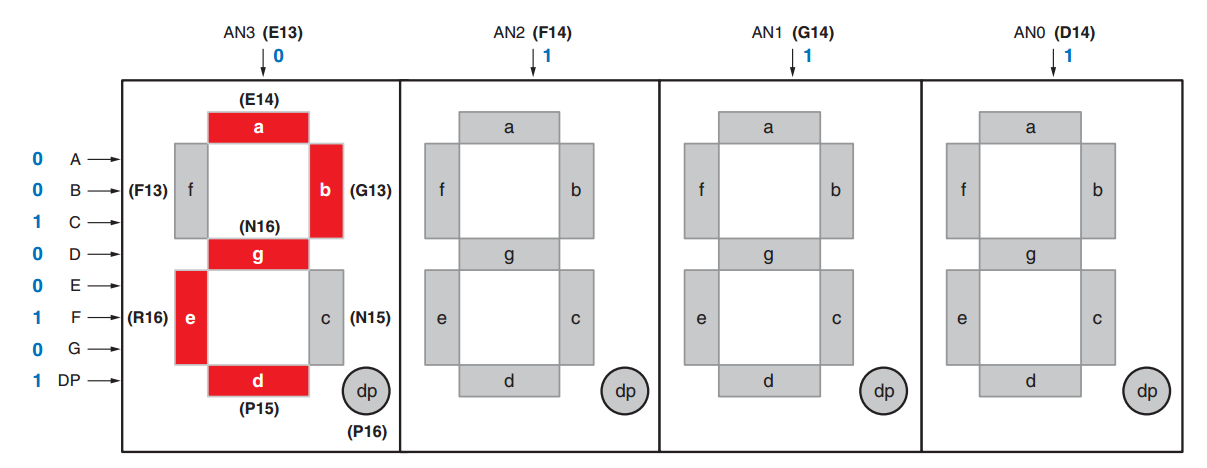
\includegraphics[width = 0.8\textwidth ]{Spartan3-7segment}}\\
                \hline
                 
            \end{tabular}
        \caption{ Salidas físicas de los displays en la Spartan-3 }
        \label{tab:tablaSalidas7Segmentos}
    \end{table}

    \begin{table}[H]
            \centering
            \begin{tabular}{|c|c|c|c|c|}
                \hline
                \rowcolor[rgb]{0.21,0.69,0.87}\multicolumn{5}{|c|}{  \textbf{ {Ánodos de control}}} \\
                \hline \hline
                \textbf{  Anodo Control  } & AN3 & AN2 & AN1 & AN0  \\
                \hline
                \textbf{  FPGA Pin  } & E13 & F14 & G14 & D14  \\
                \hline
                 
            \end{tabular}
        \caption{ Ánodos control (activos a nivel bajo) para los display de 7 segmentos }
        \label{tab:anodoControl}
    \end{table}

    Las entradas correspondientes a los \textbf{interruptores} se pueden ver en la siguiente tabla. Estos interruptores se encuentran representados con el número 11 en la figura (\ref{fig:Spartan3TopSide}) del apartado (\ref{subsection:Spartan-3}).

    \begin{table}[H]
            \centering
            \begin{tabular}{|c|c|c|c|c|c|c|c|c|}
                \hline
                \rowcolor[rgb]{0.21,0.69,0.87}\multicolumn{9}{|c|}{  \textbf{ {Entradas Interruptores}}} \\
                \hline \hline
                \textbf{  Interruptor  } & SW7 & SW6 & SW5 & SW4 & SW3 & SW2 & SW1 & SW0 \\
                \hline
                \textbf{  FPGA Pin  } & K13 & K14 & J13 & J14 & H13 & H14 & G12 & F12 \\
                \hline
                 
            \end{tabular}
        \caption{ Entradas físicas de los interruptores en la Spartan-3 }
        \label{tab:tablaEntradasInterruptores}
    \end{table}

    Los pines de entrada correspondientes a los \textbf{pulsadores} se pueden ver en la siguiente tabla. Estos componentes se corresponden con los representados con el número 13 en la figura (\ref{fig:Spartan3TopSide}) del apartado (\ref{subsection:Spartan-3}).

    \begin{table}[H]
            \centering
            \begin{tabular}{|c|c|c|c|c|}
                \hline
                \rowcolor[rgb]{0.21,0.69,0.87}\multicolumn{5}{|c|}{  \textbf{ {Entradas Pulsadores}}} \\
                \hline \hline
                \textbf{  Pulsador  } & BTN3 (Reset) & BTN2 & BTN1 & BTN0  \\
                \hline
                \textbf{  FPGA Pin  } & L14 & L13 & M14 & M13  \\
                \hline
                 
            \end{tabular}
        \caption{ Entradas físicas de los pulsadores en la Spartan-3 }
        \label{tab:tablaEntradasPulsadores}
    \end{table}

%    Por ahora no utilizamos los LEDs, queda comentado por si volvemos a usarlos.
%
%    Como se ha dicho en el apartado (\ref{subsection:Spartan-3}) la placa incorpora ocho LEDs, representados con el número 12 en la figura (\ref{fig:Spartan3TopSide}). A continuación se muestra la correlación de cada LED con la patilla de la FPGA:

%   \begin{table}[H]
%            \centering
%            \begin{tabular}{|c|c|c|c|c|c|c|c|c|}
%                \hline
%                \rowcolor[rgb]{0.21,0.69,0.87}\multicolumn{9}{|c|}{  \textbf{ {Salidas LED}}} \\
%                \hline \hline
%                \textbf{  LED  } & LD7 & LD6 & LD5 & LD4 & LD3 & LD2 & LD1 & LD0 \\
%                \hline
%                \textbf{  FPGA Pin  } & P11 & P12 & N12 & P13 & N14 & L12 & P14 & K12  \\
%                \hline
%                 
%            \end{tabular}
%        \caption{ Salidas físicas de los LEDs en la Spartan-3 }
%        \label{tab:tablaSalidasLED}
%    \end{table}

\subsection{Estructura de la memoria e información útil}

    En los siguientes apartados de la memoria se puede encontrar la explicación detallada del funcionamiento y codificación de la lógica del ascensor descrito, concretamente:
    \begin{itemize}
        \item Apartado \ref{section:DiagBloques}: Se detalla el funcionamiento interno de cada entidad o arquitectura así como su interfaz. A su vez se describe la relación entre las diferentes entidades
        \item Apartado \ref{section:Codigo}: Se adjunta la programación de cada entidad o arquitectura así como su correspondiente testbech.
        \item Apartado \ref{section:PruebasYResultados}: Se comentan los aspectos prácticos de como se ha cargado esta información en la FPGA así como los resultados obtenidos.
        \item Apéndice \ref{app:codEntSal}: Se adjuntan las tablas donde se especifica la codificación que se ha utilizado para el funcionamiento interno del ascensor.
    \end{itemize}
    
    Todo el proyecto, tanto el documento en código \LaTeX\  como los ficheros VHDL se pueden encontrar en Github \faGithub\ en el siguiente enlace: https://github.com/enheragu/Elevator-VHDL
